\documentclass[10pt,twocolumn]{article}
\ifdefined\pdftexversion\pdfoutput=1\fi  % arXiv: force pdflatex path (guarded so XeTeX/tectonic still compiles)

% ---------------------------------------------------------------------------
% Local Coding-Model Configurations on a Single DGX Spark
% arXiv preprint source. Primary category: cs.SE; cross-list cs.PF, cs.LG.
% Build: pdflatex main && pdflatex main   (no bibtex needed; bibliography is inline)
% ---------------------------------------------------------------------------

\usepackage[utf8]{inputenc}
\usepackage[T1]{fontenc}
\usepackage{lmodern}
\usepackage[margin=1in]{geometry}
\usepackage{graphicx}
\usepackage{booktabs}
\usepackage{array}
\newcolumntype{L}[1]{>{\raggedright\arraybackslash}p{#1}}
\usepackage{listings}
\lstset{%
  basicstyle=\ttfamily\scriptsize,
  breaklines=true,
  breakatwhitespace=false,
  columns=fullflexible,
  keepspaces=true,
  frame=single,
  framesep=3pt,
  xleftmargin=3pt,
  showstringspaces=false,
  postbreak=\mbox{\textcolor{gray}{$\hookrightarrow$}\space},
}
\usepackage{amsmath}
\usepackage{amssymb}
\usepackage{xcolor}
\usepackage{caption}
\usepackage[hidelinks]{hyperref}
\usepackage{xurl}  % allow long URLs to break anywhere (bibliography)
\usepackage{microtype}

\captionsetup{font=small,labelfont=bf}
\graphicspath{{figures/}}

% Compact typewriter for the many paths/flags this paper references.
\newcommand{\code}[1]{\texttt{\small #1}}

% Two-column layout tuning: let columns end naturally (no stretched inter-section
% gaps), and pin floats to the top of any float-only page instead of centering them.
\raggedbottom
\makeatletter
\setlength{\@fptop}{0pt}     % single-column floats: top of float page
\setlength{\@dblfptop}{0pt}  % full-width (table*/figure*) floats: top of float page
\makeatother

% Float placement: without these, the full-width Fig.~1 (figure*) blocks the FIFO
% float queue and every later [t] float backs up behind it, flushing only at the
% pre-appendix \clearpage -- which dumped all seven figures after the bibliography.
% Relaxing the per-page float limits lets floats settle near their citing text.
\setcounter{topnumber}{4}
\setcounter{totalnumber}{6}
\setcounter{dbltopnumber}{4}
\renewcommand{\topfraction}{0.95}
\renewcommand{\dbltopfraction}{0.95}
\renewcommand{\textfraction}{0.05}
\renewcommand{\floatpagefraction}{0.85}
\renewcommand{\dblfloatpagefraction}{0.80}
\usepackage{placeins}  % \FloatBarrier to keep section floats within their section

% Let TeX stretch a line by up to this much before overfull/badness-10000; combined
% with microtype this clears the badly spaced pinned-digest paragraph (F10).
\emergencystretch=2em

\title{\bfseries Local Coding-Model Configurations\\ on a Single DGX Spark:\\
A Systems and Methodology Case Study}

\author{Mani Malarvannan \\ \small\href{mailto:mani.malarvannan@cdw.com}{mani.malarvannan@cdw.com} \\ \small\url{https://github.com/mani-mal/spark-coder-bench}}
\date{}

\begin{document}
\maketitle

\begin{abstract}
We report a reproducible case study of serving and evaluating three open-weight
Mixture-of-Experts (MoE) coding models locally on a single NVIDIA DGX Spark
(GB10, consumer Grace Blackwell, \code{sm\_121a}, 128\,GB unified memory):
gpt-oss-120b~\cite{gptoss} (MXFP4, vLLM), Qwen3-Coder-30B-A3B~\cite{qwen3} (bf16, vLLM), and
NVIDIA Nemotron-3-Super-120B-A12B~\cite{nemotron} (NVFP4, TensorRT-LLM). This is deliberately
\emph{not} a model-ranking paper. On this hardware each model couples to exactly one
serving runtime, one quantization, and one agent scaffold, so every score describes
a \emph{deployment configuration}, not intrinsic model quality. Our contributions are
three: (1) a serving-feasibility matrix for GB10---the headline result is negative and
structural: no model in our set serves on both available runtimes, which makes a
matched same-model cross-runtime comparison infeasible on this box; (2) a three-layer
local evaluation harness (SWE-bench Verified agentic repair on a disclosed ARM64-buildable
subset, a from-scratch full-stack app build scored by an automated API contract, and
LiveCodeBench single-shot generation) with full raw-artifact retention and deterministic
rescoring; and (3) a set of measurement lessons drawn from concrete failures.
The sharpest lesson is a single harness-validity error that compressed a real
${\sim}4\times$ performance gap into an apparent statistical tie until it was found and
corrected. A second is a fixed token budget that materially depressed the observed score of a
verbose reasoning model that is competitive on the problems it answered with code. At local-evaluation scale,
serving feasibility and harness validity dominate model effects; we argue these deserve
first-class attention alongside leaderboard numbers.
\end{abstract}

\section{Motivation}

Running capable coding agents locally and privately, on hardware that sits under a desk
rather than in a datacenter, is an increasingly common goal. The DGX Spark---GB10 silicon,
128\,GB of unified LPDDR5x memory---is a plausible box for it, and 120B-class open-weight
coding models are now available in quantized forms that nominally fit. What is
under-documented is the gap between ``nominally fits'' and ``actually serves and can be
measured honestly.'' This study answers a narrow, defensible question rather than a broad
comparative one:

\begin{quote}
What serving, measurement, and evaluation constraints arise when three pinned open-weight
model configurations are run locally on one DGX Spark, and what does that imply for
reproducible coding-agent benchmark design?
\end{quote}

We make three contributions. First, a \textbf{serving-feasibility matrix} for
GB10/\code{sm\_121a}: which model/quantization/runtime combinations start successfully, and
why the others do not. Second, a \textbf{three-layer local evaluation harness} with
complete raw-artifact retention and one-command deterministic rescoring, so every number in
this paper regenerates from committed outputs without re-serving a model. Third, a set of
\textbf{measurement lessons}---most sharply, a documented case where one missing
specification file changed a headline conclusion, and a fixed token budget that depressed a
reasoning model's score in a way that looked like a capability gap but was an output-length
artifact.

We state the framing plainly because it governs how every result should be read. Model
identity on this box is fully confounded with serving runtime, quantization, and agent
scaffold, and that confound is a consequence of hardware, not a design choice we could
relax. The closest available model-versus-model comparison is the quality axis between the
two models that share a runtime (gpt-oss and Qwen, both on vLLM); even this is not a clean
contrast, since the two still differ in size, quantization (MXFP4 vs.\ bf16), architecture,
and tool/reasoning handling, so we frame it as the closest available comparison rather than a
controlled one. Everything that ties a model to a distinct runtime is a configuration
comparison and is labeled as such at the point of every affected number.

\section{Related Work}

\textbf{Coding-agent benchmarks.} SWE-bench~\cite{swebench} and its human-filtered
SWE-bench Verified subset established repository-level, execution-graded bug repair as the
dominant agentic-coding measure; a patch is scored by whether the repository's own
\code{FAIL\_TO\_PASS} and \code{PASS\_TO\_PASS} test suites pass after it is applied. We use
SWE-bench Verified as our Layer~1 anchor. LiveCodeBench~\cite{livecodebench} provides
time-windowed, single-shot competitive-programming problems with hidden tests, designed to
control contamination by selecting problems released after a model's training cutoff; we use
it as our Layer~3 single-shot code-generation axis. Because our fixed pre-2024-06 window
predates the training cutoffs of all three models, we describe it as a contamination-possible
historical window rather than a contamination-free one. Contamination-hardened and
capability-broadened successors such as SWE-bench Pro~\cite{swebenchpro} and cloud-sandboxed
agentic suites exist, but they are x86- or cloud-bound and thus off-thesis for a local, on-box study; we
treat them as related and future work rather than running them. Our Layer~2---building a
full-stack application from a frozen specification and scoring it against an automated HTTP
contract---occupies a long-horizon ``construct from nothing'' axis that few coding-agent
benchmarks test.

\textbf{Local serving of MoE models.} vLLM~\cite{vllm} and TensorRT-LLM~\cite{trtllm} are the
two OpenAI-compatible serving stacks we use. Sparse MoE architectures~\cite{switch} decouple
total parameters from per-token active parameters, which is what makes 120B-class models
tractable on a 128\,GB box; the three models here span an active-parameter fraction (active
divided by total parameters) of 4.4\% to 10.8\%. Low-bit weight formats---OCP microscaling
MXFP4~\cite{mxfp4} and NVIDIA's distinct NVFP4~\cite{nvfp4}---shrink the memory footprint
further. A recurring and under-reported subtlety, which our results make concrete, is that in
the pinned runtime builds we tested on consumer Blackwell (\code{sm\_121a}), FP4 weights were
served through weight-only kernels rather than an FP4 \emph{compute} path, so the realized FP4
benefit was storage and bandwidth, not tensor-core arithmetic. This is a property of the
software path we observed on these runtime builds, not a statement about the GB10 tensor
cores, which do support FP4 arithmetic.

\textbf{Evaluation methodology.} Our statistical treatment uses Wilson score
intervals~\cite{wilson} for binomial rates and McNemar's test~\cite{mcnemar} for paired
comparisons on shared task sets. The broader point we contribute to---that measured scores
are highly sensitive to harness details, sample size, and token budgets---is consistent with
the wider reproducibility literature, but we ground it in specific, reproducible failures on
this hardware rather than in the abstract.

\section{Experimental Setup}

\begin{figure*}[t]
\centering
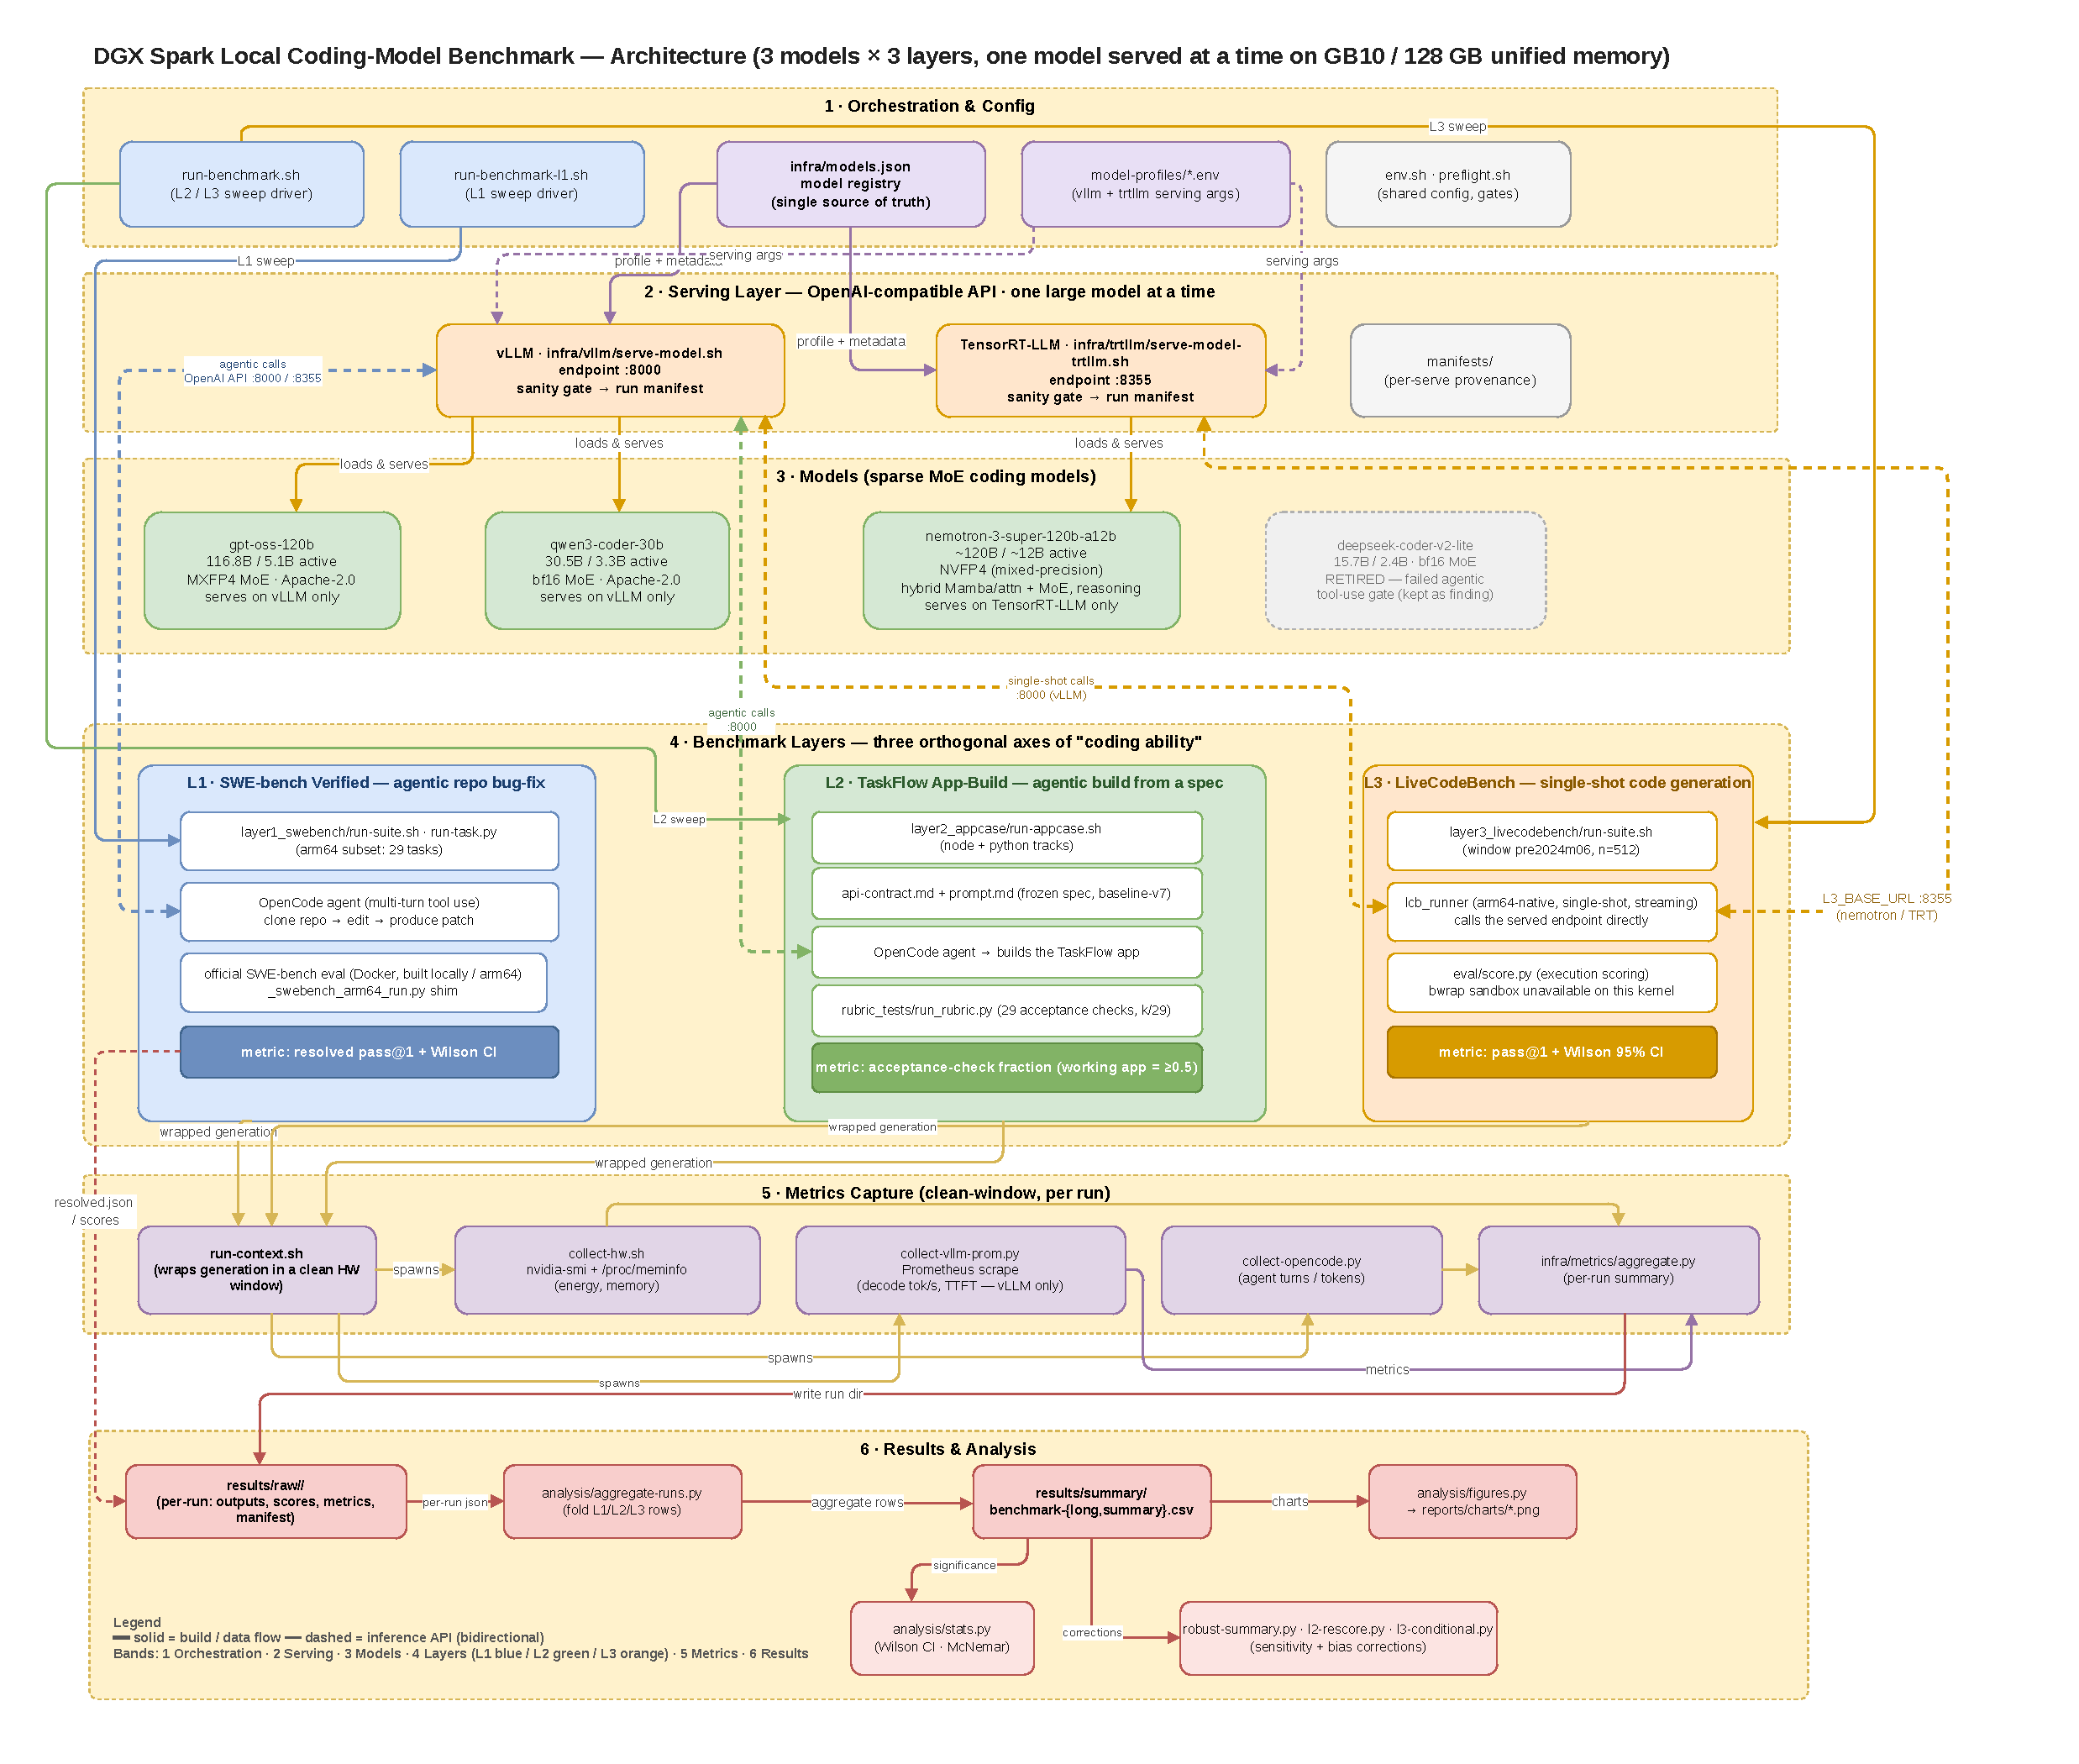
\includegraphics[width=0.92\textwidth]{architecture.pdf}
\caption{End-to-end architecture of one benchmark run on a single DGX Spark. Sweep drivers read
a single model registry and hand each arm its model plus serving profile; the selected model
comes up behind an OpenAI-compatible endpoint (vLLM on \code{:8000} or TensorRT-LLM on
\code{:8355}) after a sanity gate and a per-serve reproducibility manifest; OpenCode drives the
two agentic layers (L1, L2) while L3 calls the endpoint directly; synchronized collectors capture
hardware energy/memory, vLLM Prometheus throughput, and agent accounting into per-run summaries
that aggregate into the committed CSVs behind every table here.}
\label{fig:arch}
\end{figure*}

\subsection{Hardware}

The box is a single DGX Spark~\cite{dgxspark}: GB10, aarch64, consumer Grace Blackwell,
compute capability \code{sm\_121a}, with 128\,GB of unified LPDDR5x shared between CPU and
GPU at roughly 273\,GB/s---about $6\times$ lower than discrete Blackwell's
${\sim}1.7$\,TB/s. Decode is therefore memory-bandwidth-bound, and this shapes several
results. Software: driver 580.159.03, CUDA 13.0, device reported as \code{NVIDIA GB10}. One
large model is served at a time.

A hardware detail that matters for measurement: because memory is unified, \code{nvidia-smi}
runs correctly but its \code{memory.*} fields return \code{Not Supported}/\code{[N/A]} by
design---there is no separate VRAM pool to count. The model's memory footprint is therefore
read from \code{/proc/meminfo} as host RAM and must not be interpreted as dedicated GPU
memory. This is a property of the platform, not a broken tool, and we disclose it wherever a
memory figure appears.

\subsection{Serving and agent}

Models are served behind OpenAI-compatible endpoints: vLLM on port \code{8000} and
TensorRT-LLM on port \code{8355}. Each serve passes a correctness gate (a fixed prompt must
produce coherent, non-repeating output; a failed gate aborts the run rather than recording
garbage metrics) and writes a per-serve reproducibility manifest. Container image digests
are pinned: vLLM \code{nvcr.io/nvidia/vllm:26.02-py3} (vLLM 0.15.1) and TensorRT-LLM
\code{nvcr.io/nvidia/tensorrt-llm/release:1.3.0rc9}. The agentic layers are driven by
OpenCode~\cite{opencode} 1.17.9 at an identical version and configuration for every model;
Layer~3 uses no agent
and calls the endpoint directly.

\subsection{The three configurations}

\begin{table*}[t]
\centering
\caption{The three deployment configurations. Model identity is coupled to quantization,
runtime, and scaffold by hardware necessity, and each coupling is disclosed. No model in the
set serves on both runtimes on this box.}
\label{tab:configs}
\small
\setlength{\tabcolsep}{4pt}
\begin{tabular}{@{}L{0.13\textwidth}L{0.16\textwidth}L{0.11\textwidth}L{0.10\textwidth}L{0.09\textwidth}L{0.30\textwidth}@{}}
\toprule
Model & Architecture & Total / Active & Quant & Serves on & Why locked to one runtime \\
\midrule
gpt-oss-120b & MoE (128 exp, top-4) & 116.8B / 5.1B & MXFP4 & vLLM only &
  MXFP4 MoE autotunes on TRT-LLM but deadlocks at the executor handoff \\
nemotron-3-super & MoE-hybrid Mamba/attn & ${\sim}$120B / ${\sim}$12B & NVFP4 (mixed) & TRT-LLM only &
  vLLM 0.15.1 (\code{26.02-py3}) rejects its \code{MIXED\_PRECISION} checkpoint \\
qwen3-coder-30b & MoE (128 exp, top-8) & 30.5B / 3.3B & bf16 & vLLM only &
  bf16 MoE has no working \code{sm\_121a} TRT-LLM kernel \\
\bottomrule
\end{tabular}
\end{table*}

Table~\ref{tab:configs} lists the three arms. All are sparse MoE models with an
active-parameter fraction of 4.4\% (gpt-oss), 10.0\% (nemotron), and 10.8\% (qwen). Serving
settings cannot be equalized across all three arms, and we do not claim they are. Random seed
(\code{0}) and sampling temperature are held identical across all three arms at the serving
layer, but only the two vLLM arms (gpt-oss, qwen) additionally share KV-cache dtype policy,
\code{max\_num\_seqs}, and the OpenCode and vLLM versions. The nemotron arm runs on
TensorRT-LLM and necessarily differs: FP8 KV cache, a serving batch of 8 (against
\code{max\_num\_seqs 1} for the vLLM arms), distinct reasoning/tool parsers, and---at
Layer~1/2---MTP speculative decoding; its Layer~3 generation additionally ran 8-way
concurrently rather than single-stream. We therefore report per-configuration serving settings
(Appendix~\ref{app:serve}) rather than a single equalized protocol, and label every
cross-runtime comparison as a configuration comparison. What no arm equalizes is disclosed
throughout: quantization, serving runtime, and \code{max\_model\_len}/memory-utilization under
the 128\,GB ceiling.

A candidate fourth model, DeepSeek-Coder-V2-Lite, was evaluated and retired before any timed
run. It generates correct code but, in the tested configuration, did not \emph{autonomously}
call tools---in an OpenCode smoke test it claimed success while writing nothing to disk---so it
could not drive the agent loop. We introduced an explicit autonomous-tool-use gate as a precondition for the agentic
layers: a model must return a well-formed \code{tool\_calls} response under
\code{tool\_choice:"auto"} (not prose, not hallucinated tool-output tokens) \emph{and}
actually create a file on disk (Appendix~\ref{app:gate}). gpt-oss-120b passed this gate and replaced DeepSeek. The case
is itself a finding: agentic competence is not the same property as code-generation
competence, and a benchmark that conflates them will mis-rank models.

\subsection{The headline systems result: serving feasibility}
\label{subsec:serving}

The single most practitioner-useful finding is negative and structural. \textbf{No model in
our set serves on both runtimes on GB10/\code{sm\_121a}.} Nemotron is TensorRT-LLM-only:
vLLM 0.15.1 as shipped in NGC \code{26.02-py3} rejects its checkpoint at configuration
validation, before any weights load. The checkpoint declares
\code{quant\_algo=MIXED\_PRECISION} (FP8 on the Mamba mixer projections, NVFP4 on the MoE
experts, per layer, produced by ModelOpt 0.43.0.dev63), and this vLLM build's ModelOpt loader
accepts only a single uniform algorithm from a fixed whitelist. The failure is a
\code{pydantic} validation error raised in ${\sim}6$\,s during engine-config
construction, not an out-of-memory condition or a runtime crash
(Appendix~\ref{app:nemotron} gives the checkpoint quant config and the verbatim error). We scope this claim
precisely: it is a property of \emph{vLLM 0.15.1 as shipped in NGC 26.02-py3}, the stack we
pinned for driver compatibility; we did not test a newer vLLM build or the current
NVIDIA-validated DGX Spark recipe, so the claim is scoped to the pinned stack, not to vLLM in
general. A circulating workaround forces the top-level algorithm to NVFP4; we deliberately did
not use it, because the Mamba mixer projections are genuinely FP8 in the weights and forcing
NVFP4 risks silently miscasting them---a model-under-test that might load but generate subtly
wrong output is worse than one that cleanly refuses.

Conversely, the two vLLM models do not serve on TensorRT-LLM 1.3.0rc9 on this silicon: bf16
MoE has no working \code{sm\_121a} kernel, and MXFP4 MoE autotunes but then deadlocks at the
server-to-executor handoff. The consequence is that a same-model, cross-runtime ``bridge''
run---the clean way to isolate a runtime effect from a model effect---is impossible on this
box with the pinned runtimes. This is exactly why we treat the arms as configurations and
make no controlled cross-runtime speed or energy claim.

\section{Evaluation Design}

\begin{table}[t]
\centering
\caption{The three measurement layers. L1/L2 are agentic (multi-turn tool use); L3 is
single-shot. Scoring is fully automated and mechanical at every layer---no human scorers and
no LLM judge.}
\label{tab:layers}
\small
\setlength{\tabcolsep}{3pt}
\begin{tabular}{@{}p{0.10\linewidth}p{0.42\linewidth}p{0.36\linewidth}@{}}
\toprule
Layer & What & Metric \\
\midrule
L1 & SWE-bench Verified repo bug-fix, agentic & resolved pass@1 on a disclosed 29-task
ARM64-buildable subset \\
L2 & Full-stack app build from a frozen spec, agentic & automated API acceptance-check
fraction ($k/29$) \\
L3 & LiveCodeBench single-shot generation & pass@1 with Wilson 95\% CI ($n{=}512$) \\
\bottomrule
\end{tabular}
\end{table}

The three layers (Table~\ref{tab:layers}) probe orthogonal axes of ``coding ability.'' L1 and
L2 are agentic multi-turn tool use driven through OpenCode; L3 is single-shot generation
against the endpoint. Keeping them separate is deliberate: it lets ``code generation is not
the same as agentic tool use'' be an empirical observation rather than an assumption.

\textbf{Layer 1} runs on a 29-task ARM64-buildable subset of SWE-bench Verified, and we are
explicit that this is \emph{not} SWE-bench Verified performance and \emph{not} a random sample
of the full 500-instance set. The official task images are x86-only. Rather than probe all
500 instances, we drew a stratified sample of up to four instances from each of the 12
SWE-bench Verified repositories (43 instances in total), built each one's environment natively
for aarch64, and kept the 29 whose environment builds and whose gold patch resolves on ARM64.
This is an empirical buildability probe over a stratified sample---not the full buildable set,
and not a curated difficulty sample; two of the 12 probed repositories (xarray, scikit-learn)
failed to build on aarch64 and contribute no tasks. The surviving subset is biased toward
pure-Python repositories (flask, requests, pylint, pytest, sympy, sphinx, and similar) and
excludes anything needing x86-only wheels or heavy C/Fortran toolchains---a coverage
limitation we disclose. Because all three configurations run the identical ARM64-built tasks,
any ARM-versus-x86 environment difference cancels in the relative comparison. The subset, the
43-instance probe list, and their checksums are pinned in the provenance record; the
surviving 29 tasks and their per-repository distribution are listed in Appendix~\ref{app:subset}.

\textbf{Layer 2} has each model build the same realistic full-stack application (``TaskFlow
Local'') from an identical frozen specification, across a Node.js and a Python/FastAPI backend
track. Scoring fires 29 equally weighted, fully automated HTTP assertions against a frozen API
contract after booting the built app, reported as an acceptance-check fraction $k/29$. This is
an API-acceptance signal, not a holistic app-quality score: it measures whether the app boots
and satisfies the communicated contract, not user experience, design, or maintainability. We
report a Bernoulli working-app rate---a run counts as a working app if the built app boots and
passes at least half of the 29 checks ($k/29 \ge 0.5$)---with a Wilson interval as the
headline, never a single-$N$ mean rubric score. We label the 0.5 cutoff exploratory, and note
that the 29 checks are stateful and mutually dependent (later checks reuse state created by
earlier ones) rather than independent Bernoulli trials.

\textbf{Layer 3} runs LiveCodeBench single-shot on a fixed pre-2024-06 window of 512 problems,
scored as pass@1 with a Wilson 95\% interval. A shared maximum generation budget of 8192
tokens is held identical across all three models as a fairness control---a decision that turns
out to be consequential (Section~\ref{sec:l3}).

\textbf{Scoring and fairness.} Scoring is deterministic given the retained artifacts, so runs
can be rescored from committed outputs without re-serving. Same spec, prompt, hardware, time
box, and harness for every run; all serving-setting differences that could not be equalized
are disclosed; the maintainer's tooling never edits model-generated application code, which
lives in a separate repository.

\section{Results}

Figure~\ref{fig:quality} shows success by layer with Wilson intervals. On raw scores the
ordering is gpt-oss $\ge$ qwen $\ge$ nemotron, but the L1 and L2 gaps are statistically weak
and the L3 nemotron gap is budget-confounded. We report the numbers and then explain, layer by
layer, why the durable finding is about how one measures rather than which model wins.

\begin{figure}[t!]
\centering
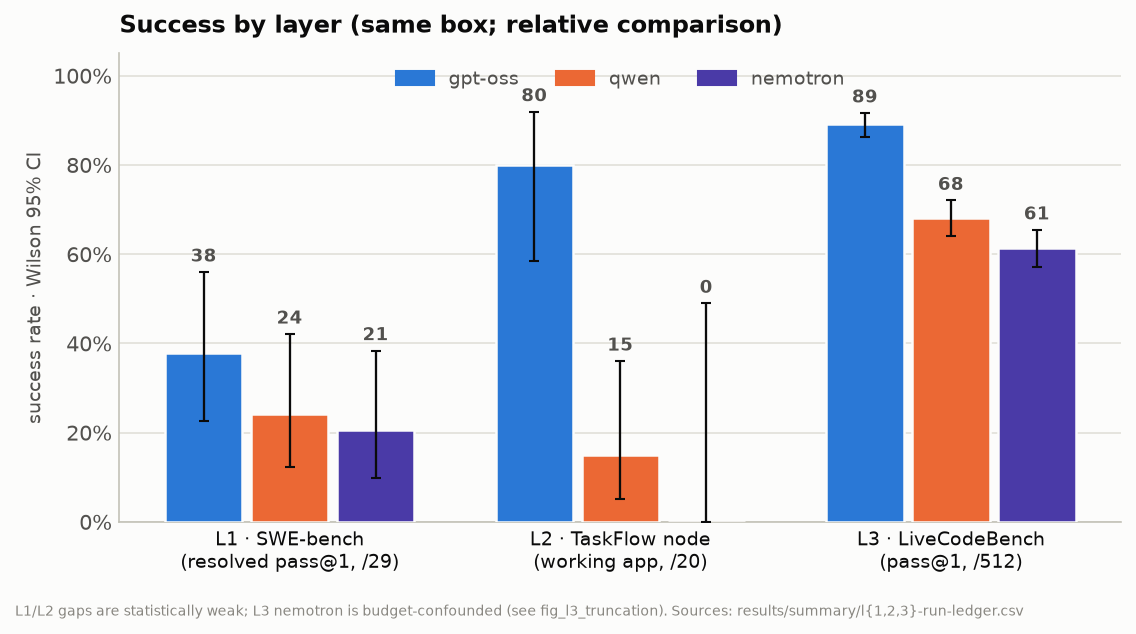
\includegraphics[width=\linewidth]{quality-by-layer.png}
\caption{Success by layer for the three configurations, each with a Wilson 95\% interval:
L1 resolved pass@1, L2 node working-app rate, L3 pass@1. The raw ordering is
gpt-oss $\ge$ qwen $\ge$ nemotron, but the L1/L2 separations are weak and the L3 nemotron
result is a token-budget artifact (Figure~\ref{fig:trunc}).}
\label{fig:quality}
\end{figure}

\subsection{Layer 1: SWE-bench Verified ARM64 subset}

\begin{table*}[t]
\centering
\caption{Layer 1, 29-task ARM64 subset, single-attempt pass@1. The raw $k/29$ rate is primary
(intention-to-treat); the ``model-valid'' rate, which excludes operational failures (a watchdog
kill and eight clone/DNS/guard-drops that were never a measured attempt) from the denominator,
is reported only as a sensitivity analysis.}
\label{tab:l1}
\small
\begin{tabular}{@{}lccc@{}}
\toprule
Model & Resolved (raw) & Model-valid rate & Notes \\
\midrule
gpt-oss-120b & 37.9\% (11/29) & 37.9\% (11/29) & no infra failures \\
qwen3-coder-30b & 24.1\% (7/29) & 24.1\% (7/29) & no infra failures \\
nemotron-super & 20.7\% (6/29) & 30.0\% (6/20) & 1 watchdog kill; 8 excluded \\
\bottomrule
\end{tabular}
\end{table*}

Table~\ref{tab:l1} gives the Layer~1 rates. Two points about denominators. First, the primary
rate we report is the raw, intention-to-treat $6/29 = 20.7\%$: it charges every operational
failure (a watchdog kill and eight environment failures---clone/DNS/guard drops---that were
never a measured model attempt) against the configuration. As a sensitivity analysis we also
report a model-valid rate that excludes those nine non-attempts, $6/20 = 30.0\%$; we flag it as
a sensitivity rather than the headline because excluding failures from only one arm can
introduce selection bias, and watchdog/runtime failures may themselves be
configuration-dependent. Second, pairwise McNemar tests on the shared 29 tasks find no
significant separation for any pair, before or after a Holm correction across the three
comparisons: gpt-oss vs.\ nemotron $p = 0.125$ (Holm-adjusted $0.375$), gpt-oss vs.\ qwen
$p = 0.289$ (adjusted $0.578$), and nemotron vs.\ qwen $p = 1.0$ (adjusted $1.0$). At this
sample size the layer cannot rank these models; we read this as a failure to reject, not as
evidence of equivalence.

A second axis matters beyond ``did it fix the bug.'' SWE-bench also records whether a patch
broke something that previously passed (\code{PASS\_TO\_PASS}). Among patches that applied and
were evaluated, gpt-oss regresses at least one previously-passing test 33.3\% of the time
(8/24), qwen 31.8\% (7/22), and nemotron 21.4\% (3/14). The severity diverges far more than the
rate: gpt-oss broke 1078 \code{PASS\_TO\_PASS} tests to nemotron's 3, because a few catastrophic
patches (for instance, breaking an import so a whole module's suite fails) dominate the count.
Figure~\ref{fig:regression} shows the trade-off: gpt-oss's aggressive edits resolve the most and
regress the most, while nemotron's fewer, smaller edits rarely regress but rarely resolve. This
characterizes failure quality among the non-resolving runs, not the winners, and the small
denominators keep it directional.

\begin{figure}[t!]
\centering
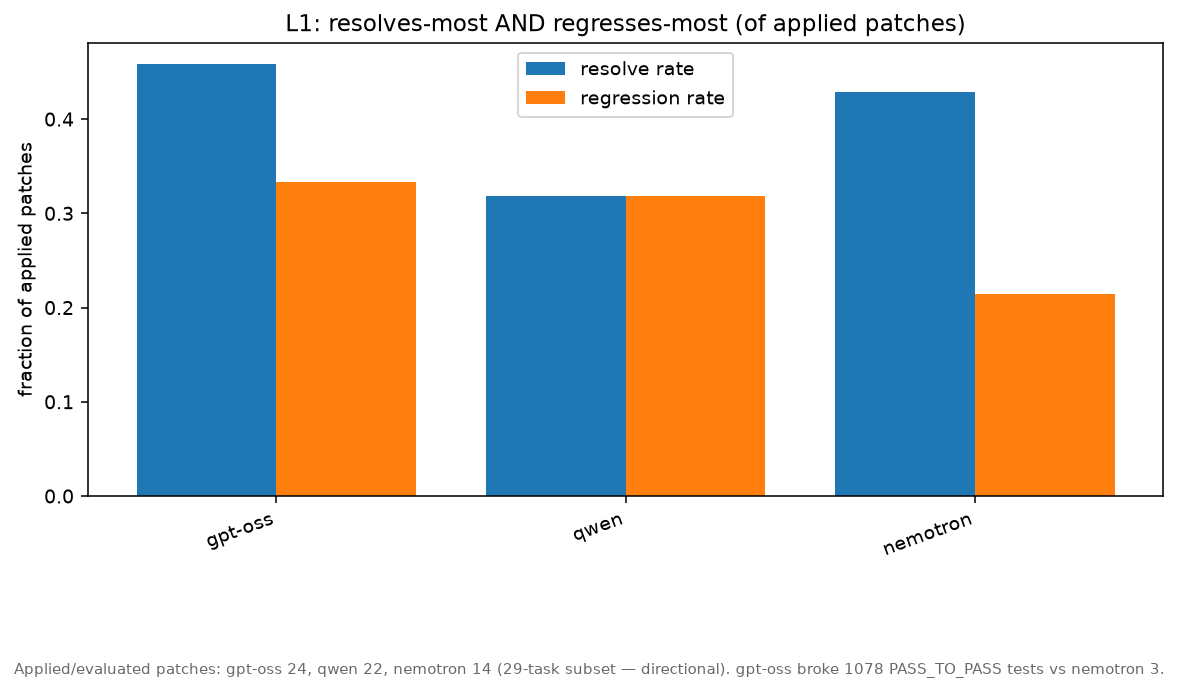
\includegraphics[width=\linewidth]{regression-rate.png}
\caption{Layer 1 collateral damage, as a fraction of applied patches. gpt-oss both resolves the
most and regresses the most; nemotron regresses least but resolves little. Aggressive editing
buys resolutions at the cost of regressions.}
\label{fig:regression}
\end{figure}

\subsection{Layer 2: app-build acceptance, and a harness bug that changed the conclusion}
\label{subsec:l2}

The first Layer~2 sweep was produced under a harness-validity error we label C1. The frozen API
contract that the prompt requires the model to satisfy had been dropped from the workspace by an
app-repository tag-lineage break: four of the 29 checks were structurally unreachable, and every
model was graded against a contract it could not see. After restoring the contract (app-repo tag
\code{baseline-v7}) and re-running the vLLM models, the picture changed decisively.

\begin{table*}[t]
\centering
\caption{Layer 2 after the C1 contract fix (contract-visible \code{baseline-v7}) for the two
vLLM arms. Working-app rate counts a run that boots and passes at least half of the 29 checks; the
python $k/29$ column gives the mean acceptance fraction with the working-app count in
parentheses (zero for both). The nemotron row (starred) is a pre-C1 measurement that was
\emph{not} rerun; it is shown for reference only and is not comparable to the corrected rows.}
\label{tab:l2}
\small
\begin{tabular}{@{}lccc@{}}
\toprule
Model & node $k/29$ & node working & python $k/29$ \\
\midrule
gpt-oss-120b & 0.724 & 16/20 = 80\% & 0.069 (0/8) \\
qwen3-coder-30b & 0.178 & 3/20 = 15\% & 0.004 (0/8) \\
nemotron-super$^\ast$ & 0.009 (N=4) & 0/4 & 0.000 (N=4) \\
\bottomrule
\end{tabular}
\end{table*}

Table~\ref{tab:l2} reports the corrected sweep. Under the bug, gpt-oss (node acceptance 0.252)
and qwen (0.155) looked indistinguishable---the working-app Wilson intervals overlapped, and the
honest read was ``too close to call.'' Corrected, gpt-oss (node acceptance 0.724)
substantially outperforms qwen (0.178) on the node track: 80\% working apps
(16/20, Wilson 95\% $[58.4, 91.9]\%$) against 15\% (3/20, $[5.2, 36.0]\%$), and the
working-app intervals no longer overlap. We report this descriptively: the 20 runs per cell are repeated
trials of a single application specification, not 20 independent tasks, and the harness applies
no inferential test at Layer~2, so we make no population-level significance claim. (Were the
runs treated as independent, a Fisher exact test on the node working-app counts would give
$p \approx 9\times10^{-5}$; we report it only to bound the effect, not as a validated result.)
The before/after are also two separate stochastic sweeps rather than a contemporaneous
controlled A/B, so we describe the change as observed, not as a clean causal isolation.
Crucially, the contract helped \emph{only where a model could already build a booting app}:
gpt-oss's node score rose $2.9\times$ (the four contract-only checks, marked in
Appendix~\ref{app:contract}, went from 0 to 48 passes),
while qwen and both python tracks, which are floored for other reasons, barely moved. A single
missing specification file had compressed a roughly $4\times$ performance gap on this task into
an apparent statistical tie. Figure~\ref{fig:ablation} shows the before/after.

\begin{figure}[t!]
\centering
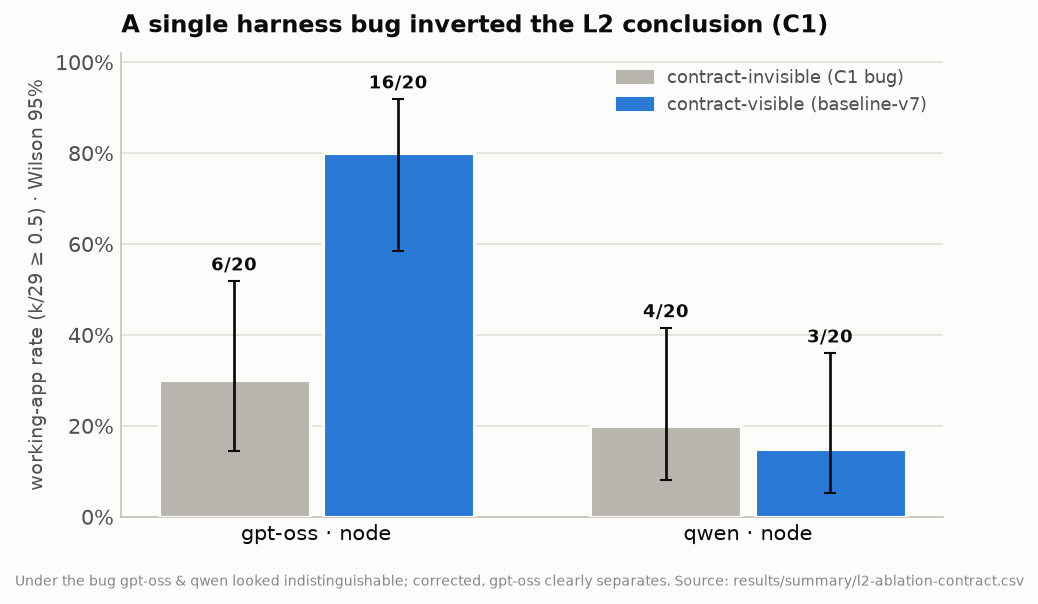
\includegraphics[width=\linewidth]{l2-contract-ablation.png}
\caption{The C1 ablation. Under the harness bug (contract invisible), gpt-oss (6/20) and qwen
(4/20) working-app rates overlap. With the contract restored, gpt-oss jumps to 16/20 while qwen
stays flat and the intervals separate. One missing spec file changed the observed conclusion
(before/after are separate stochastic sweeps, not a contemporaneous A/B).}
\label{fig:ablation}
\end{figure}

The asterisk on nemotron marks an asymmetry we disclose explicitly. Nemotron was \emph{not}
rerun with the visible contract, so its row is a pre-C1 measurement---retained and marked, but
not comparable to the corrected vLLM rows. We did not rerun it because at Layer~2 it almost
never produced a working backend (node acceptance mean 0.009, zero working apps) and the four
contract-only checks require a booted backend to be reachable; we judged a rerun a poor use of
fragile TensorRT-LLM compute, but we do not claim to have measured that the contract would have
no effect on it. For the vLLM models, results are dual-reported as $k/29$ and a C1-rescored
$k/25$ over the 25 reachable checks (gpt-oss node 0.744, qwen 0.184). Two caveats survive the
correction: the python track floors for both vLLM models, a genuine node-versus-python asymmetry
rather than a contract artifact; and the layer remains an API-acceptance signal, not a full
app-quality score.

\subsection{Layer 3: LiveCodeBench, and a token budget that manufactured a last place}
\label{sec:l3}

\begin{table*}[t]
\centering
\caption{Layer 3 LiveCodeBench pass@1 (pre-2024-06 window, $n{=}512$). Nemotron's raw rate is
depressed by output truncation under the shared 8192-token budget (see text). The no-code column
counts problems with empty output or no extractable code block, all scored as fails.}
\label{tab:l3}
\small
\begin{tabular}{@{}lccc@{}}
\toprule
Model & pass@1 & Wilson 95\% CI & no-code (of 512) \\
\midrule
gpt-oss-120b & 89.3\% & [86.3, 91.7] & 7 (1.4\%) \\
qwen3-coder-30b & 68.2\% & [64.0, 72.1] & 10 (2.0\%) \\
nemotron-super & 61.3\% & [57.0, 65.4] & 185 (36.1\%) \\
\bottomrule
\end{tabular}
\end{table*}

Table~\ref{tab:l3} gives raw Layer~3 pass@1, where nemotron finishes last. That last place is
substantially driven by output truncation under the shared 8192-token budget: nemotron's verbose
reasoning left 185 of 512 problems with no extractable code (143 empty outputs plus 42 with
output but no code block), all scored as fails, against 7/512 for gpt-oss and 10/512 for qwen.
Whether a larger budget would recover correct answers on those 185 problems was not measured, so
we report the truncation itself rather than an imputed higher score. The truncation is
difficulty-correlated---no-code rate 14.3\% on easy, 34.3\% on medium, 71.5\% on hard
problems---so a rate conditional on only the answered subset must not be compared against the
other models' full-512 rates, a selection-bias trap we flag (finding C2). As a conditional
analysis, on the 327 problems nemotron answered with code---an easier subset selected by
nemotron's own behavior, so this is accuracy \emph{conditional on emitting extractable code} and
is not comparable to the full-set rates---nemotron scores 96.0\% (314/327), gpt-oss 95.4\%
(312/327), and qwen 82.3\% (269/327). The primary Layer~3 score for every model remains the
full-set rate in Table~\ref{tab:l3}. Figure~\ref{fig:trunc} shows both halves.

\begin{figure}[t!]
\centering
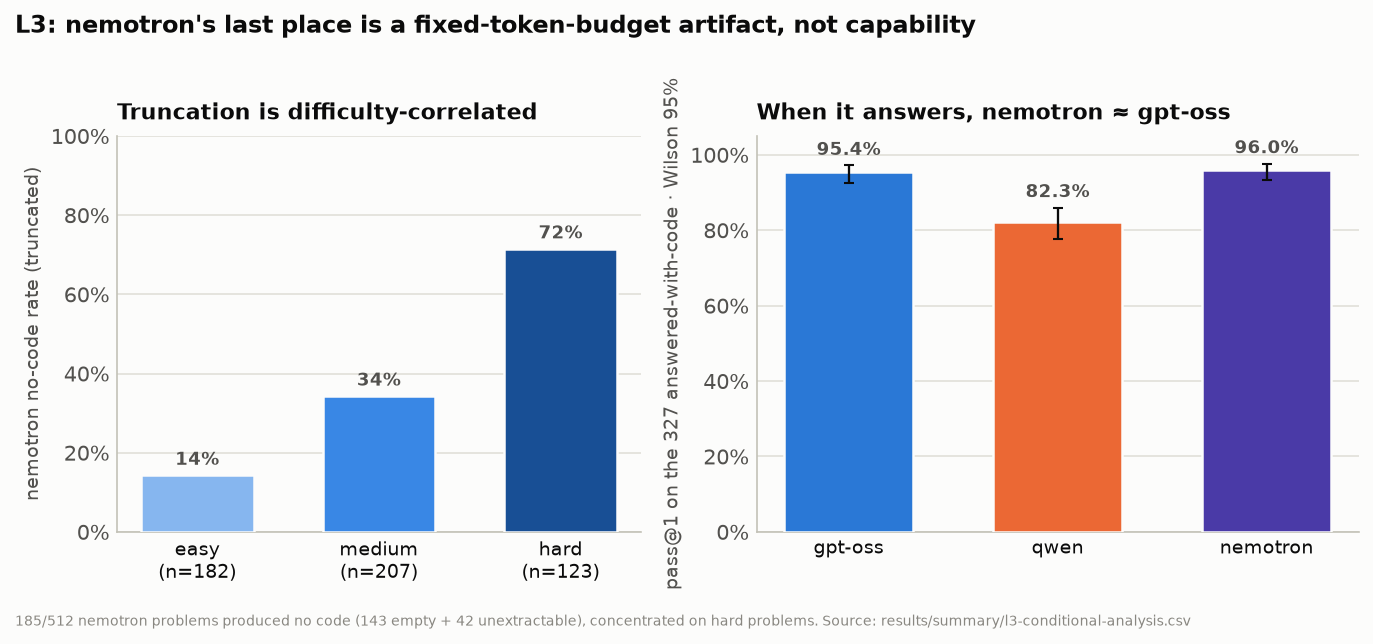
\includegraphics[width=\linewidth]{l3-truncation.png}
\caption{Left: nemotron's no-code (truncation) rate rises with difficulty (easy 14\%, medium
34\%, hard 72\%). Right: on the 327 problems it answers with code---a conditional, easier subset,
not comparable to full-set rates---nemotron scores 96.0\%, gpt-oss 95.4\%, and qwen 82.3\%. Much
of nemotron's last place in Table~\ref{tab:l3} reflects truncation under the fixed budget rather
than incorrect answers.}
\label{fig:trunc}
\end{figure}

The methodology finding is general: a single-shot, fixed-budget benchmark systematically
penalizes verbose reasoning models, and the penalty concentrates on hard problems. We keep 8192
tokens as the primary, controlled number---holding the budget constant is the fairness
control---and treat the truncation itself as a reportable result rather than tuning it away.

\section{Measurement Pitfalls}
\label{sec:pitfalls}

Several pitfalls surfaced only because we retained raw artifacts and re-derived every table.
They generalize beyond this box.

\textbf{Unified memory is not VRAM.} As noted, \code{nvidia-smi} reports \code{[N/A]} for
device memory on GB10 by design; the footprint comes from \code{/proc/meminfo} and is
whole-system, not dedicated GPU memory.

\textbf{Tokens-per-joule is prompt-token-dominated.} The agent loop re-sends context every
turn, so prompt tokens are a median 98.7\% of the total. A naive \code{total\_tokens / energy}
therefore measures re-submitted context, not decode work; we report energy per \emph{generated}
token alongside it.

\textbf{Restart-truncated energy windows.} Watchdog restarts reuse a run identifier and
overwrite the metric window, so a crash-prone run's energy can cover only its final segment.
The gpt-oss Layer~3 energy cell is a known-broken capture (roughly three orders of magnitude
low) and is marked invalid in the ledger rather than published---the pass@1 result is
unaffected because scoring is independent of the metrics window.

\textbf{Robust energy statistics.} Arithmetic-mean Layer~1 energy is dominated by a single
${\sim}13$\,h nemotron operational runaway (${\sim}655$\,kJ). We report median and IQR
with an operational-failure sensitivity, never a bare mean.

\textbf{Telemetry asymmetry.} vLLM exposes Prometheus histograms (gpt-oss ${\sim}26.9$\,tok/s,
qwen ${\sim}19.7$\,tok/s at Layer~1, decode-throughput means; the per-task medians in
Table~\ref{tab:resource} are 26.2 and 20.1); TensorRT-LLM exposes none, so nemotron has hardware
energy but no decode-throughput or TTFT figures. Those cells are blank by design, not missing
data, and we do not impute them.

\section{Operational Findings}

A few operational notes for anyone reproducing this. TensorRT-LLM 1.3.0rc9 on GB10 is
fragile for non-NVIDIA MoE models---the FP4-native NVIDIA reasoning model serves, the others
deadlock. A degraded-box state is real: after a 26-hour vLLM run the GPU was left in a state
where TensorRT-LLM nemotron wedged after one generation (warm-up 656\,s); a reboot restored
normal operation (warm-up back to 8\,s), so the box should be reset between heavy long-lived
serves. A non-streaming request path wedged nemotron mid-generation, and switching the
LiveCodeBench runner to stream (the path OpenCode already used) fixed it. Throughput is
bandwidth-bound: nemotron's single-stream Layer~3 was estimated at ${\sim}130$\,h (a
full-budget-decode extrapolation, not a measured single-stream run), so we ran it 8-way
concurrently (${\sim}9.5$\,h measured). We did not run a 1-way-versus-8-way sensitivity check, so we
disclose this concurrency difference as a further configuration confound rather than assert it is
quality-neutral; pass@1 is scored per problem and independent of the metrics window, and
TensorRT-LLM exposes no throughput/energy histograms to lose. Finally, several silent-failure
traps were guarded: reasoning
models return \code{content=None} on truncation; a resume filter re-generated empty outputs
indefinitely; and a watchdog nearly false-stalled on a frozen log mtime and now uses the
TensorRT-LLM iteration counter as ground truth. Figures~\ref{fig:walltime} and
\ref{fig:energy} summarize the efficiency reality, with the caveats above embedded, and
Appendix~\ref{app:resource} (Table~\ref{tab:resource}) consolidates the per-model, per-layer
resource medians.

\begin{figure}[t!]
\centering
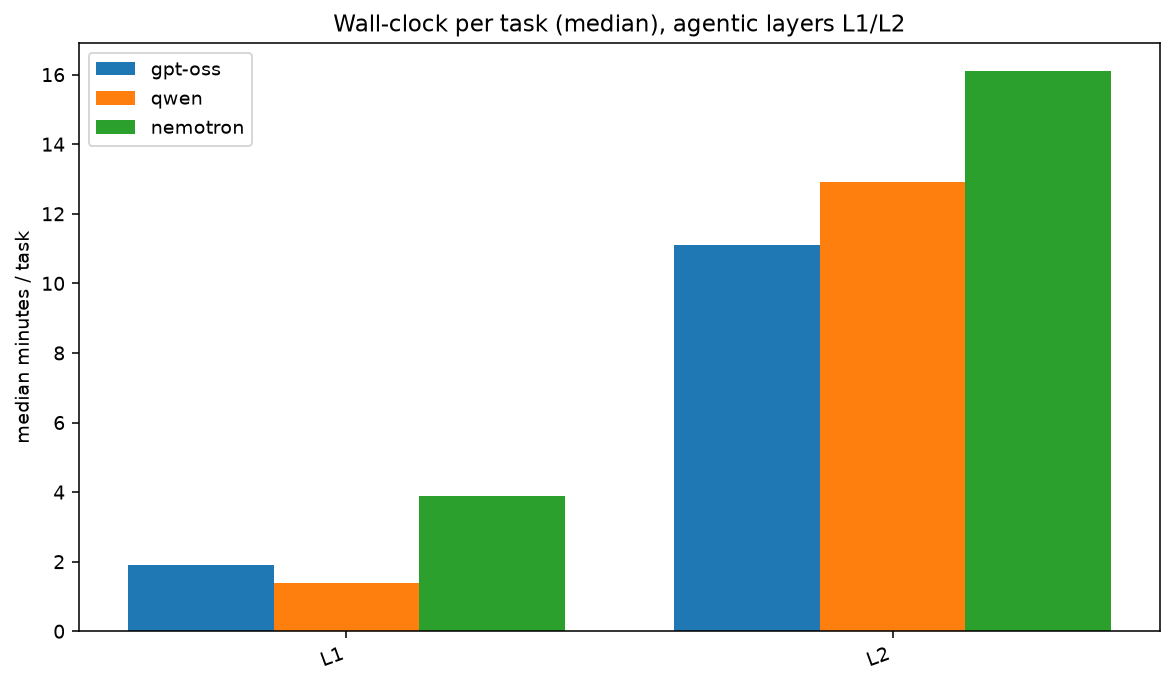
\includegraphics[width=\linewidth]{walltime-by-layer.png}
\caption{Median wall-clock per task, agentic layers. Nemotron is roughly $2\times$ slower than
the vLLM models at L1 (3.9 vs 1.4--1.9\,min) and slowest at L2 (16.1\,min); the median is shown
because the L1 mean is skewed by one ${\sim}13$\,h runaway.}
\label{fig:walltime}
\end{figure}

\begin{figure}[t!]
\centering
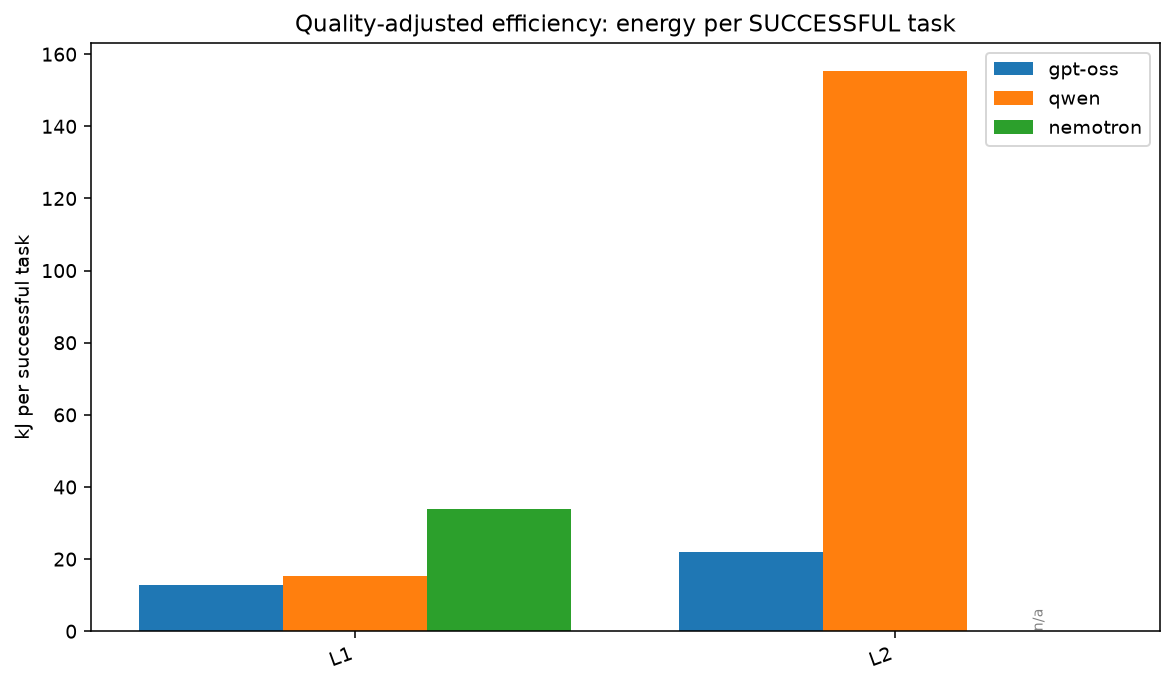
\includegraphics[width=\linewidth]{energy-per-success.png}
\caption{Energy per \emph{successful} task (GPU-reported \code{nvidia-smi} \code{power.draw},
GPU package only, no idle subtraction; runtime-confounded, nemotron on TensorRT-LLM). At L1,
nemotron costs ${\sim}33.8$\,kJ per solve---over its 20 model-valid energy windows, excluding
one ${\sim}13$\,h watchdog runaway (${\sim}655$\,kJ, 76\% of its L1 energy)---to gpt-oss's
12.8\,kJ (${\sim}2.6\times$); including the runaway inflates it to 143\,kJ. At L2, energy per
working app is Node-track only (all working apps are Node): qwen 155.3\,kJ to gpt-oss's
22.1\,kJ; pooling in the Python track, which produced no working apps, inflates these to 211 and
32.8\,kJ.}
\label{fig:energy}
\end{figure}

\section{Reproducibility}

Every run keeps its summaries, manifests, and clock records under
\code{results/raw/<run-id>/}; bulky per-run time series are regenerable and excluded from
version control, while summaries and manifests are committed. Scoring is fully automated and
mechanical---no human scorers, no LLM judge, at any layer---so the aggregation and robust-summary
scripts regenerate their numeric tables deterministically from retained outputs (rendered figures
may differ bytewise across matplotlib/toolchain versions, but the underlying values do not). A
single command
(\code{make rebuild}) re-derives the summary tables, per-run ledgers, figures, and statistics from
the raw runs---without re-serving any model, and excepting one frozen pre/post ablation artifact
whose pre-fix sweep was not retained---and the statistics and robust-summary self-tests pass.
Container image digests, upstream dataset snapshot revisions (SWE-bench Verified, LiveCodeBench),
the exact HuggingFace revisions of all three model checkpoints, the Layer~1 subset checksums, and
the frozen Layer~3 window are pinned in an immutable provenance record. Model-generated
application code lives only in the companion app repository and is never edited by the
maintainer's tooling; the coding assistant used to build the harness and write this report is not
part of what was measured.

\section{Threats to Validity and Limitations}

\textbf{Single box, three configurations.} Model identity is fully coupled to serving runtime,
precision, and scaffold. Conclusions are restricted to these configurations on this machine, and
serving incompatibility is a systems finding, not proof of intrinsic quality.

\textbf{Small and unequal samples.} L1 and L3 are single-attempt per cell; L2 is $N=20/8$
(node/python) for the vLLM models against $N=4$ for nemotron. All quality claims are descriptive,
and the McNemar results show L1 cannot rank these models at this size.

\textbf{Protocol changed mid-collection.} The C1 contract fix and rubric-denominator changes mean
some early runs are exploratory; confirmatory claims draw on the post-fix \code{baseline-v7}
sweep.

\textbf{L1 is a disclosed subset,} 29 tasks kept from a 43-instance stratified (up-to-four-per-repo)
buildability probe, not SWE-bench Verified, not the full ARM64-buildable set, and not a random
sample of the 500 instances; absolute SWE-bench numbers should not be extrapolated from it.

\textbf{L3 is a fixed historical window} where contamination is possible: equal chronological
eligibility is not equal contamination, the set is not exposure-balanced, and it is not
leaderboard-comparable.

\textbf{Untested newer stacks.} The nemotron/vLLM incompatibility is scoped to the pinned vLLM
0.15.1 (NGC \code{26.02-py3}); a newer vLLM or the current NVIDIA-validated DGX Spark recipe was
not tested and could change that specific result.

\textbf{Isolation.} Generated code is executed without OS-level sandboxing on this kernel
(bubblewrap unavailable); publication-grade runs should use a no-network container or VM.

\section{Conclusion}

On a single DGX Spark the story that survives scrutiny is not ``model X wins.'' It is that at
local-evaluation scale, serving feasibility and harness validity dominate model effects. No model
in our set serves on both runtimes on this box; a single missing specification file changed the
Layer~2 conclusion until it was found; and a fixed token budget substantially depressed the
Layer~3 score of a verbose reasoning model that, on the problems it answered with code, scored
comparably to the field (whether a larger budget would recover its full-set score is untested).
The practitioner takeaways are concrete. Of the configurations measured here, gpt-oss-120b on
vLLM is the strongest local agentic setup (L1 37.9\%, L2 node 80\% working apps, L3 89.3\%);
nemotron serves only on TensorRT-LLM and its Layer~3 score is heavily affected by the shared
token budget; and honest local benchmarking depends far more on a failure taxonomy, robust
energy statistics, and deterministic rescoring than on producing one more leaderboard number.

\section*{Data and Code Availability}

The harness, frozen specification, raw run summaries, aggregation and statistics code, figures,
and provenance pins are in the public repository at
\url{https://github.com/mani-mal/spark-coder-bench}. Every table and figure in
this paper maps to a committed source CSV, and all but one regenerate via \code{make rebuild};
the sole exception is the Layer~2 C1 before/after ablation (Figure~\ref{fig:ablation}), whose
pre-fix sweep was not retained in the regenerable long-form CSV, so its source table is
versioned as a committed frozen artifact. The
model-generated application code lives in the separate public companion repository
\url{https://github.com/mani-mal/taskflow-local-app-benchmark}; all reported Layer~2 runs start
from its frozen tag \code{baseline-v7} (commit \code{5b0b85b}).

\begin{thebibliography}{99}

\bibitem{swebench}
C. E. Jimenez, J. Yang, A. Wettig, S. Yao, K. Pei, O. Press, and K. Narasimhan.
\newblock SWE-bench: Can Language Models Resolve Real-World GitHub Issues?
\newblock \emph{ICLR}, 2024. arXiv:2310.06770.

\bibitem{livecodebench}
N. Jain, K. Han, A. Gu, W.-D. Li, F. Yan, T. Zhang, S. Wang, A. Solar-Lezama,
K. Sen, and I. Stoica.
\newblock LiveCodeBench: Holistic and Contamination-Free Evaluation of Large Language Models for Code.
\newblock arXiv:2403.07974, 2024.

\bibitem{vllm}
W. Kwon, Z. Li, S. Zhuang, Y. Sheng, L. Zheng, C. H. Yu, J. E. Gonzalez, H. Zhang, and I. Stoica.
\newblock Efficient Memory Management for Large Language Model Serving with PagedAttention.
\newblock \emph{SOSP}, 2023. arXiv:2309.06180.

\bibitem{trtllm}
NVIDIA.
\newblock TensorRT-LLM: A TensorRT toolbox for optimized large language model inference.
\newblock \url{https://github.com/NVIDIA/TensorRT-LLM}. Container image \code{release:1.3.0rc9}.

\bibitem{swebenchpro}
Scale AI.
\newblock SWE-bench Pro: A contamination-resistant, enterprise-grade software engineering benchmark.
\newblock 2025. \url{https://github.com/scaleapi/SWE-bench_Pro-os}.

\bibitem{switch}
W. Fedus, B. Zoph, and N. Shazeer.
\newblock Switch Transformers: Scaling to Trillion Parameter Models with Simple and Efficient Sparsity.
\newblock \emph{JMLR}, 2022. arXiv:2101.03961.

\bibitem{wilson}
E. B. Wilson.
\newblock Probable Inference, the Law of Succession, and Statistical Inference.
\newblock \emph{Journal of the American Statistical Association}, 22(158):209--212, 1927.

\bibitem{mcnemar}
Q. McNemar.
\newblock Note on the Sampling Error of the Difference Between Correlated Proportions or Percentages.
\newblock \emph{Psychometrika}, 12(2):153--157, 1947.

\bibitem{opencode}
OpenCode.
\newblock OpenCode: an open-source terminal-based coding agent. Version 1.17.9.
\newblock \url{https://opencode.ai}.

\bibitem{gptoss}
OpenAI.
\newblock gpt-oss-120b \& gpt-oss-20b Model Card.
\newblock arXiv:2508.10925, 2025. Card: \url{https://huggingface.co/openai/gpt-oss-120b}.

\bibitem{qwen3}
Qwen Team.
\newblock Qwen3-Coder-30B-A3B-Instruct model card.
\newblock \url{https://huggingface.co/Qwen/Qwen3-Coder-30B-A3B-Instruct}, 2025.

\bibitem{nemotron}
NVIDIA.
\newblock NVIDIA-Nemotron-3-Super-120B-A12B-NVFP4 model card.
\newblock \url{https://huggingface.co/nvidia/NVIDIA-Nemotron-3-Super-120B-A12B-NVFP4}, 2026.

\bibitem{mxfp4}
Open Compute Project.
\newblock OCP Microscaling Formats (MX) Specification, Version 1.0.
\newblock \url{https://www.opencompute.org/documents/ocp-microscaling-formats-mx-v1-0-spec-final-pdf}, 2023.
\newblock See also B. Rouhani et al., Microscaling Data Formats for Deep Learning, arXiv:2310.10537, 2023.

\bibitem{nvfp4}
NVIDIA.
\newblock Introducing NVFP4 for Efficient and Accurate Low-Precision Inference.
\newblock NVIDIA Technical Blog, 2025.
\newblock \url{https://developer.nvidia.com/blog/introducing-nvfp4-for-efficient-and-accurate-low-precision-inference/}.

\bibitem{dgxspark}
NVIDIA.
\newblock NVIDIA DGX Spark (GB10 Grace Blackwell): product specifications.
\newblock \url{https://www.nvidia.com/en-us/products/workstations/dgx-spark/}, 2025.

\end{thebibliography}

\clearpage
\appendix

\section{Serving Commands and Configurations}
\label{app:serve}

Both runtimes are launched from a single sequential driver that writes a per-serve
reproducibility manifest and passes a coherence sanity gate before any timed run. The vLLM
invocation (Qwen shown; per-model values come from the \code{infra/models.json} registry, and
\code{--max-num-seqs 1} is pinned across all models for clean per-task latency):

\begin{lstlisting}
docker run -d --name vllm-server --gpus all --ipc=host \
  --network=host --ulimit memlock=-1 --ulimit stack=67108864 \
  -v $HF_HOME:/root/.cache/huggingface \
  nvcr.io/nvidia/vllm:26.02-py3 \
  vllm serve Qwen/Qwen3-Coder-30B-A3B-Instruct \
    --host 0.0.0.0 --port 8000 --served-model-name qwen3-coder-30b \
    --gpu-memory-utilization 0.80 --max-model-len 65536 \
    --max-num-seqs 1 --max-num-batched-tokens 16384 \
    --dtype auto --trust-remote-code --seed 0 \
    --enable-auto-tool-choice   # + per-profile tool-call parser
\end{lstlisting}

TensorRT-LLM serves Nemotron on port \code{8355} with an \code{extra\_llm\_api\_options} YAML.
The 1.3.0rc9 image is required: 1.2.1's \code{nemotron\_h} loader fell back to a regular init
and double-allocated to ${\sim}115$\,GB, OOM-ing the host.

\begin{lstlisting}
trtllm-serve nvidia/NVIDIA-Nemotron-3-Super-120B-A12B-NVFP4 \
  --host 0.0.0.0 --port 8355 \
  --max_batch_size 8 --tp_size 1 --ep_size 1 \
  --max_num_tokens 8192 --max_seq_len 1048576 \
  --extra_llm_api_options /config/nemotron-super.yaml \
  --reasoning_parser nano-v3 --tool_parser qwen3_coder
\end{lstlisting}

The run-time serving values above come from the committed per-serve manifests
(\code{max\_batch\_size 8}, \code{max\_seq\_len 1048576}---the 1M sequence length is feasible
because the KV cache is FP8). The Layer~3 profile is identical except that MTP speculative
decoding is disabled (a KV-manager wedge under MTP, documented in the findings), so the
\code{speculative\_config} block below applies to Layers~1--2 only.

The YAML encodes the 128\,GB unified-memory strategy for this hybrid Mamba/attention MoE
(FP8 KV cache, float16 SSM cache with stochastic rounding, chunked prefill):

\begin{lstlisting}
kv_cache_config:
  dtype: fp8
  enable_block_reuse: false
  free_gpu_memory_fraction: 0.9
  mamba_ssm_cache_dtype: float16
  mamba_ssm_stochastic_rounding: true
moe_config:
  backend: CUTLASS
cuda_graph_config:
  enable_padding: true
  max_batch_size: 8
enable_chunked_prefill: true
speculative_config:
  decoding_type: MTP
  num_nextn_predict_layers: 3
\end{lstlisting}

\section{The Nemotron vLLM Rejection}
\label{app:nemotron}

This is the headline serving-feasibility result of Section~\ref{subsec:serving}. The checkpoint's
\code{hf\_quant\_config.json} (produced by \code{modelopt 0.43.0.dev63}) declares a
\emph{mixed-precision} format---FP8 on the Mamba mixer projections, NVFP4 on the MoE experts,
specified per layer:

\begin{lstlisting}
{ "quantization": {
    "quant_algo": "MIXED_PRECISION",
    "kv_cache_quant_algo": "FP8",
    "quantized_layers": {
      "backbone.layers.0.mixer.in_proj":  {"quant_algo": "FP8"},
      "backbone.layers.0.mixer.out_proj": {"quant_algo": "FP8"},
      "backbone.layers.1.mixer.experts.0.up_proj":
          {"quant_algo": "NVFP4", "group_size": 16},
      "...": "~every MoE expert listed, NVFP4 group_size 16"
} } }
\end{lstlisting}

vLLM 0.15.1's ModelOpt loader accepts only a single uniform algorithm and rejects the model
during \code{create\_engine\_config(...)}---in ${\sim}6$\,s, before any weight loads, and
before any tool/reasoning-parser flag is reached:

\begin{lstlisting}
pydantic_core._pydantic_core.ValidationError: 1 validation
  error for VllmConfig
  Value error, ModelOpt currently only supports:
  ['FP8', 'FP8_PER_CHANNEL_PER_TOKEN', 'FP8_PB_WO', 'NVFP4']
  quantizations in vLLM. Please check the
  `hf_quant_config.json` file for your model's quant config.
\end{lstlisting}

No profile or parser change fixes this: the rejected value is the checkpoint's own format. A
circulating workaround forces the top-level field to \code{NVFP4}; we did not use it, because
the Mamba mixer projections are genuinely FP8 in the weights and forcing NVFP4 risks silently
miscasting them. The same error against the same model and container is filed upstream at
\code{vllm-project/vllm\#37854} and \code{NVIDIA/dgx-spark-playbooks\#77}.

\section{The Autonomous Tool-Use Gate}
\label{app:gate}

Before any timed agentic run, a model must pass a two-part gate; a model that fails is reported
as a non-agentic baseline rather than scored as if it tried. (1) A direct request to the served
endpoint with \code{tool\_choice:"auto"} and a tool schema must return a non-null, well-formed
\code{tool\_calls} object---not prose, and not hallucinated tool-output tokens in the content.
(2) In an OpenCode smoke test the model must actually create a file on disk. A model that only
acts under \code{tool\_choice:"required"} fails part (1). This is the gate DeepSeek-Coder-V2-Lite
failed---it generated correct code but wrote nothing to disk while reporting success---and that
gpt-oss-120b passed before replacing it.

\section{Layer 2 API Contract}
\label{app:contract}

Layer 2 scores 29 equally weighted, fully automated HTTP assertions after booting the built
app. The checks and their categories:

\begin{lstlisting}
boot:     health_ok
auth:     login_admin_ok, login_bad_creds_401,
          me_without_token_401, me_with_token_200,
          login_member_ok
security: user_no_password_field,
          protected_route_no_token_401
rbac:     member_create_project_403
projects: admin_create_project, project_list_contains,
          project_get_by_id, project_edit*, project_archive*
tasks:    task_create, task_list, task_get,
          task_update_status*, task_filter_status,
          task_search, task_delete
comments: comment_add, comment_list
validation: validation_project_no_name_400,
          validation_task_no_title_400,
          validation_task_bad_priority_400
dashboard: dashboard_summary_keys*
frontend: frontend_build
reproducibility: lockfile_present
\end{lstlisting}

The four checks marked \code{*} are the C1 contract-only assertions of Section~\ref{subsec:l2}: they pin
exact routes and key sets the requirements prose leaves unspecified, so they are reachable only
when the frozen \code{api-contract.md} is in the workspace. Each check is a small deterministic
assertion; the RBAC bypass check---which caught apps that let a non-admin member create a
project---is representative:

\begin{lstlisting}
# member (non-admin) must be forbidden from creating a project
r, _ = self.req("POST", C.API + "/projects",
                token=member_token, json={"name": "X"})
self.add("member_create_project_403", "rbac",
         r is not None and r.status_code == 403,
         r.status_code if r else "none")
\end{lstlisting}

\section{Layer 1 ARM64-Buildable Subset}
\label{app:subset}

The 29 tasks are the SWE-bench Verified instances that built natively on aarch64 and whose gold
patch resolved there, drawn from a 43-instance stratified probe (up to four instances from each
of the 12 SWE-bench Verified repositories)---an empirical buildability probe, not the full
buildable set and not a difficulty sample. Ten of the 12 probed repositories contributed at least
one surviving task; neither xarray nor scikit-learn built on aarch64. The distribution across the
surviving repositories:

\begin{table}[h]
\centering\small
\begin{tabular}{@{}lc lc@{}}
\toprule
Repository & N & Repository & N \\
\midrule
astropy   & 4 & pylint    & 3 \\
django    & 3 & pytest    & 4 \\
matplotlib& 2 & requests  & 4 \\
seaborn   & 2 & sphinx    & 2 \\
flask     & 1 & sympy     & 4 \\
\bottomrule
\end{tabular}
\end{table}

\begin{lstlisting}
astropy__astropy-12907  astropy__astropy-13033
astropy__astropy-13236  astropy__astropy-13398
django__django-10554    django__django-10880
django__django-10914    matplotlib__matplotlib-13989
matplotlib__matplotlib-14623  mwaskom__seaborn-3069
mwaskom__seaborn-3187   pallets__flask-5014
psf__requests-1142      psf__requests-1724
psf__requests-1766      psf__requests-1921
pylint-dev__pylint-4551 pylint-dev__pylint-4661
pylint-dev__pylint-4970 pytest-dev__pytest-10051
pytest-dev__pytest-10081 pytest-dev__pytest-10356
pytest-dev__pytest-5262 sphinx-doc__sphinx-10449
sphinx-doc__sphinx-10466 sympy__sympy-11618
sympy__sympy-12096      sympy__sympy-12419
sympy__sympy-12481
\end{lstlisting}

\section{Per-Model, Per-Layer Resource Metrics}
\label{app:resource}

Table~\ref{tab:resource} gives the consolidated hardware figures behind the efficiency
discussion. Nemotron's decode-throughput and TTFT cells are blank because TensorRT-LLM exposes
no Prometheus histograms (Section~\ref{sec:pitfalls}), not because the data is missing. Layer 3 is omitted here:
its duration is a whole-run figure rather than per-task, and the gpt-oss L3 metrics window
failed to capture the generation (Section~\ref{sec:pitfalls}). Energy and wall-clock are per-task medians;
memory is peak unified (system) RAM.

\begin{table*}[t]
\centering
\caption{Per-model, per-layer resource metrics (medians). Source:
\code{results/summary/perf-resource-summary.csv}. One gpt-oss L2 run lacks a resource-metrics
window, so its $N{=}27$ against the 28 node+python runs elsewhere.}
\label{tab:resource}
\footnotesize
\setlength{\tabcolsep}{4pt}
\begin{tabular}{@{}llcccccccc@{}}
\toprule
Layer & Model & N & min/task & kJ/task & GPU util \% & GPU W & peak mem (MiB) & decode tok/s & TTFT p50 (s) \\
\midrule
L1 & gpt-oss-120b    & 29 & 1.9 & 3.6 & 90.7 & 30.1 & 113{,}059 & 26.2 & 0.47 \\
L1 & qwen3-coder-30b & 29 & 1.4 & 2.6 & 89.3 & 29.2 & 110{,}455 & 20.1 & 0.50 \\
L1 & nemotron-super  & 21 & 3.9 & 8.4 & 91.8 & 38.0 & 108{,}517 & --   & --   \\
L2 & gpt-oss-120b    & 27 & 11.1 & 18.8 & 88.5 & 30.8 & 111{,}132 & 31.0 & 0.36 \\
L2 & qwen3-coder-30b & 28 & 12.9 & 21.5 & 92.7 & 27.7 & 110{,}250 & 22.8 & 0.21 \\
L2 & nemotron-super  &  8 & 16.1 & 40.6 & 90.6 & 45.3 & 107{,}594 & --   & --   \\
\bottomrule
\end{tabular}
\end{table*}

\end{document}
